\documentclass[10pt,twocolumn]{article}
\usepackage[utf8]{inputenc}
\usepackage{geometry}
\usepackage{graphicx}
\usepackage{amsmath,amssymb}
\usepackage{hyperref}

\geometry{
  top=0.65in,
  bottom=0.65in,
  left=1in,
  right=1in
}

\title{\textbf{Multimodal Eureka: Rewards Generated by LLM with Additional Visual Input}}
\author{
\begin{tabular}{cc}
     \textbf{Łukasz Łopacki} & \textbf{Szymon Pobłocki} \\
     Unversity of Warsaw & University of Warsaw \\
     ll439936@students.mimuw.edu.pl & s.poblocki@student.uw.edu.pl
     \\\\
     \textbf{Paweł Siwak} & \textbf{Jakub Winiarski} \\
     Unversity of Warsaw & University of Warsaw \\
     pl.siwak@student.uw.edu.pl & jj.winiarski@student.uw.edu.pl
     \\\\
     \textbf{Konrad Staniszewski\footnote{First supervisor}}  & \textbf{Paweł Budzianowski\footnote{Second supervisor}}\\
     University of Warsaw & University of Warsaw\\
     ks.staniszewski@uw.edu.pl & budzianowski@gmail.com
\end{tabular}
}
\date{\today}

\begin{document}

\maketitle

\begin{center}
    {\Large\bfseries Abstract}
\end{center}

\begin{center}
\begin{minipage}{0.90\linewidth}
\small

Eureka is a recent framework where large language models generate reward functions for reinforcement learning agents using only code-level environment descriptions. We want to extend this approach by introducing \textbf{Multimodal Eureka}, which supplements the model with visual input to improve its intuitive understanding of tasks. This mimics how humans better comprehend situations when both visual and textual information are available. We plan on evaluating our method on several control environments, assesing whether visual context can lead to higher-quality rewards and improved success rates in complex tasks.

\end{minipage}
\end{center}

\section{Introduction}
Large language models have demonstrated impressive capabilities as semantic planners for high-level decision-making tasks. Recently, effort has been made to utilise them for low-level motor control—such as dexterous manipulation and precision tasks—remains. One example of such work is the Eureka framework \cite{eureka} that addresses part of this gap by using LLMs to automatically generate and evolve reward functions through in-context learning and evolutionary optimization.

Eureka has been shown to outperform human-crafted rewards on 83\% of 29 benchmark tasks, including several involving hand-based control, without requiring task-specific templates or prior tuning. Despite its success, Eureka operates exclusively on internal state inputs (e.g., joint angles, velocities), which limits its effectiveness in tasks where visual perception plays a central role.

In many real-world robotic applications, visual input is essential for interacting with objects in unstructured environments, resolving occlusions, and aligning actions based on external context. To address this limitation, we propose to extend Eureka with visual capabilities—enabling it to generate and refine reward functions based on visual observations in addition to internal state.

We call this extension \textbf{Multimodal Eureka}. Our approach augments the reward design process with visual inputs by leveraging multimodal large language models capable of interpreting both code and image data. While most relevant information can theoretically be inferred from environment code and variable names, we hypothesize that visual representations help the model build a more intuitive understanding of the task—similarly to how a human benefits from seeing a situation rather than imagining it solely from description. We hypothesize that this added context can improve the model’s ability to generate more aligned and effective reward functions in tasks where spatial reasoning or object interaction plays a key role.


\section{Related Work}
Recently, increasingly powerful large language models are being developed, like OpenAI GPT-4 \cite{GPT-4} or Gemini \cite{Gemini}. One area in which such models can be utilized is robot control. In a work done at Microsoft \cite{Microsoft}, a model is prompted to steer a robot via generated code to accomplish a given task, with model having a textual description of the environment at its disposal. 

LLMs like GPT-4 now often have auxiliary capabilities, such as also accepting additional image data, which is utilized to increase the accuracy of LLMs in robot control tasks. For instance, the work \cite{TUDelft}, is a simple expansion of the previously quoted Microsoft paper, while a more recent article in Nature \cite{Nature} is a more advanced framework for steering robots, also utilizing GPT-4 with image data.

A different way to utilize LLMs for such tasks is to have them design rewards for Reinforcement Learning programs, rather than steer the robot directly. Since the publication of the seminal Eureka paper \cite{eureka}, which describes a framework for reward design many new frameworks aiming to alleviate some of Eureka's flaws have been proposed. They include frameworks such as CARD \cite{card}, which attempts to minimize token usage in comparison with Eureka, or Text2Reward \cite{Text2Reward}, which writes code for rewards directly instead of using APIs. However, to our knowledge, no attempts to supplement Eureka with image data have been made, which appears to us to be a worthwhile endeavour.

In our comparison we mainly utilized \verb|Gemma3-27B-IT| \cite{Gemma3-27B-IT} model. We also compared this model's performance with performance of models from the \verb|Gemini| family, such as \verb|Gemini 2.0 Flash-Lite| \cite{Gemini_2.0_Flash_Lite} and \verb|Gemini 2.0 Flash| \cite{Gemini_2.0_Flash}, and also \verb|Gemini 2.5 Flash| \cite{Gemini_2.5}.

\section{Method}

Our work extends the \textit{Eureka} framework by integrating multimodal, vision-based feedback into its feedback loop. The original method consists of three key elements:
\begin{enumerate}
    \item Environment as context
    \item Evolutionary search
    \item Reward reflection
\end{enumerate}

We propose \textit{Multimodal Eureka}, which uses vision to enhance the third stage and generate more robust and effective reward functions based on richer feedback. We believe that this approach should allow meaningful information to be collected in cases where this wasn't possible based solely on numerical metrics.

% something about switching to the Genesis env should be written here

\subsection{Environment as Context}

The foundational step in both \textit{Eureka} and our approach is providing the Large Language Model with the environment's source code, so it could understand the state space and dynamics of the task. This allows the LLM to generate syntactically correct and semantically relevant reward functions.

This process is crucial for two reasons:

\begin{itemize}
    \item By having direct access to the source code, particularly the class definition and observation function, the LLM learns the precise names, data types, and structures of the available state variables (e.g., \texttt{self.base\_lin\_vel} or \texttt{self.base\_pos}). This knowledge is essential for generating a reward code that is directly executable within the simulation environment and preventing common errors.
    \item The variable names and logic within the source code provide semantic clues about the task's objective. This allows the Large Language Model to compose reward functions that are not just syntactically valid, but also logically aligned with solving the task. In essence, the code grounds the LLM's high-level understanding of a concept like ``walking forward'' into the specific, computable variables of the simulation.
\end{itemize}

\subsection{Evolutionary Search}

Following the initial generation, our method adheres to \textit{Eureka's} evolutionary search algorithm to find the optimal reward function. This process involves the iterative generation, evaluation, and refinement of the reward code. First, the LLM generates a population of candidates for the reward function. Each candidate is then used to train a reinforcement learning policy for a set number of steps. The resulting policy's performance is evaluated using a fitness function, based on simulation metrics (e.g., success rate). The reward function that performed best in one iteration is used as a seed for the next, enabling the system to progressively discover more effective reward structures.

The original research paper mentions that the algorithm ``searches for
5 iterations with K = 16 samples per iteration''~\cite{eureka}. We tried to replicate this configuration as closely as possible. For each experiment, we ran five iterations of the search. Unfortunately, we were unable to replicate the setup perfectly due to limitations in computing power. Therefore, we decided to halve the batch size sampled on each iteration to be able to effectively run environments based on those generated reward functions in parallel without running out of memory.

\subsection{Reward Reflection}

The final component of \textit{Eureka} is Reward Reflection, where the LLM analyzes a summary of the policy's training dynamics to propose improvements to the reward function. This summary originally consisted of textual data, such as success rates, mean episode lengths, and the values of individual reward components over time.

\textit{Multimodal Eureka} enriches the reflection process by incorporating visual data into the feedback prompt. The textual summary is augmented with \textbf{key frames}. These are images that visualise the training process at certain stages. By providing this multimodal feedback, the LLM should be able to perform more targeted and insightful reward editing. It can directly ``see'' why a policy is failing. For example, an awkward fall or incorrect movement of limbs can be detected. Based on this, it can adjust the reward function to penalize these specific, visually identifiable behaviors. This moves beyond pure code optimization to a more holistic, visually informed process of reward design.

\section{Experiments}
The main goal of our project is to build upon ideas presented in the \textit{Eureka} paper~\cite{eureka}. We would like to leverage the multimodal abilities of current SoTA LLMs and try to get even higher efficiency than in the referenced paper.

In the original work, \textit{Eureka} was compared with L2R~\cite{l2r}, human-written rewards created by active reinforcement learning researchers, and sparse rewards (success/failure). \textbf{The main purpose of our experiments is to compare \textit{Multimodal Eureka} with the original \textit{Eureka} itself.} Because \textit{Eureka} has already been compared with the aforementioned baselines, we do not see a reason to check other baselines. We aim to achieve better results than in the original paper by leveraging the power of computer vision, particularly in terms of spatial understanding.

To check the results, we will conduct a series of experiments.

\begin{itemize}
    \item We will calculate \textit{Success Rate} for both algorithms for multiple environments. However, we probably won't include those used in the original paper (e.g. \textit{Isaac Gym}~\cite{isaac_gym}), as they're quite old, no longer maintained, and therefore hard to use. Instead, we'll try to focus on leveraging the \textit{K-Sim}~\cite{ksim_repo} RL training library for humanoid locomotion and manipulation.
    \item We will test different types of prompts for image analysis in \textit{Multimodal Eureka} and choose the best one in terms of the average \textit{Success Rate}.
    \item The experiments will probably require a large model, so our choice of LLM will depend on what we can access. We will consider using multimodal \textit{Gemini} and \textit{GPT} models.
    \item We will experiment with different numbers of input images (e.g. last few frames).
    \item We will check the impact of image quality on the \textit{Success Rate}.
\end{itemize}

Our goal is to find the best possible solution. The primary challenge lies in creating prompts that will enable the model to extract the most crucial information from the images. The second challenge is to make the solution as general as possible. The original \textit{Eureka} uses the same set of prompts for each environment, and we would like to fulfill this requirement too.

To explain to the reader what the aim of \textit{image prompts} is, let us show an example of what a simplified version of a prompt could look like:
\\\\
\texttt{Based on an input image and instructions from the initial\_system prompt~\footnote{initial\_system prompt is a fragment from source code repository~\cite{eureka_repo} describing an agent his role and expected output}, create an optimal reward function, which will allow the agent to solve the environment efficiently. Take into consideration the laws of physics and try to connect variable names from the source code with what you see in the provided pictures.}
\\\\
Different prompts can lead to various unexpected behaviors. Therefore, we will try to identify such cases and list the most interesting observations. If we get meaningful results for situations with a clear physical explanation, we will list them in the final report as well.

\section{Results and Discussion}

In this section we present results obtained both by running the \textit{Multimodal Eureka} and the original \textit{Eureka} in the aforementioned \textit{Genesis} environment. The latter were collected for two main reasons:

\begin{enumerate}
    \item To check whether we're able to reproduce the results of the original \textit{Eureka} research paper
    \item To establish a baseline and thus enable a comparison between those methods to draw reasonable conclusions
\end{enumerate}

To make the comparison fair we performed each of those experiments using the same configuration, i.e.:

\begin{itemize}
    \item 5 iterations of the algorithm loop
    \item 8 samples collected per iteration
    \item 130 RL training iterations with 64 environments running in parallel, which resulted in around 200k total time steps for each sample
\end{itemize}

The only things that changed between the experiments were the parameters being tested, such as the frequency of photo sampling or the LLM used.

\subsection{Baseline}

\subsubsection{Setup}

In order to establish a meaningful baseline, we performed a series of experiments, each using a different LLM as a backbone. For this experiment, we did not add any visual feedback to the pipeline. Essentially, we reproduced the original Eureka setup, but in a different environment and with different LLMs. The models we've tested were from Google. In particular, we used four different models:

\begin{enumerate}
    \item Gemma 3 27B
    \item Gemini 2.0 Flash-Lite
    \item Gemini 2.0 Flash
    \item Gemini 2.5 Flash
\end{enumerate}

This choice was purely pragmatic as Google offers a pretty wide range of models with decent quotas completely for free. We decided to test these four models because they seemed to be powerful enough to create effective reward functions while being sufficiently diverse (in terms of size and efficiency) for the sake of experimenting. Each of these models also has solid multimodal capabilities. We didn't test smaller models of the Gemma family because we were afraid that they wouldn't be capable of working in such a setup effectively.

\subsubsection{Results and Conclusions}

\begin{table}
    \centering
    \begin{tabular}{|l|c|}
        \hline
        Generated By              & Consecutive Successes \\
        \hline
        Gemma 3 27B               & -0.2819               \\
        Gemini 2.0 Flash-Lite     & -0.2934               \\
        Gemini 2.0 Flash          & -0.2349               \\
        Gemini 2.5 Flash          & -0.3200               \\
        \hline
    \end{tabular}
    \caption{Mean consecutive successes metric calculated from five runs of the final evaluation for each baseline experiment. Higher values are better.}
    \label{tab:baseline_results}
\end{table}

The results of the experiments performed are presented in Table \ref{tab:baseline_results}. Counterintuitively, they don't align with the idea of ``the bigger the model, the better the results''. Such results may suggest a few things.

Firstly, the variance of a single experiment can be quite high, particularly given the limited number of samples used in each iteration. Unfortunately, we didn't have enough time or computing power to perform more experiments or run larger ones.

Secondly, the definition of the consecutive successes metric may be flawed. However, we have used the same formula as the authors of the original research paper for the Anymal environment.

Another visible issue is the low values of the metric, which suggests that either the problem was too difficult for the models or we did not fit them for long enough.

To gain more insights, we decided to collect the best samples for each experiment and run the training once again, outside of the \textit{Eureka} loop, but this time for much longer (1000 iterations) and using more parallel environments (1024). We also ran a training session for an example human-shaped reward function in such a setup to see what kind of results it's gonna produce.

\begin{table}
    \centering
    \begin{tabular}{|l|c|}
        \hline
        Generated By              & Consecutive Successes \\
        \hline
        Gemma 3 27B               & -0.2732               \\
        Gemini 2.0 Flash-Lite     & -0.2924               \\
        Gemini 2.0 Flash          & -0.0980               \\
        Gemini 2.5 Flash          & -0.2539               \\
        Human                     & -0.0302               \\
        \hline
    \end{tabular}
    \caption{Final values of the extended setup of training for baseline generations. Higher values are better.}
    \label{tab:baseline_results_extended}
\end{table}

As can be seen in Table \ref{tab:baseline_results_extended}, the results changed most noticeably for the largest models, especially Gemini 2.0 Flash. This model achieved values close to those obtained when trained using a human-shaped reward function. The quadruped robot actually learnt to move forward using this generated reward. However, its movement pattern was clumsy, resembling a series of small jumps rather than a walk.

These results also show that, while larger LLMs have the potential to generate quite effective reward functions when the agent is trained for a longer time, more episodes don't significantly impact the results for smaller models. This suggests that models such as Gemma 3 27B and Gemini 2.0 Flash-Lite may be too weak for such a challenge, but this will be tested more thoroughly in further experiments.

\subsection{Multimodal LLMs Comparison}

\subsubsection{Setup}

To extend the comparison made when establishing a baseline for this project, and reasonably test whether the addition of vision actually encouraged models to produce more robust reward functions,  we decided to perform a comparison of LLM backbones also for the setup with vision included. The core configuration of the experiments remained exactly the same. In terms of visual feedback, we decided to collect 5 images per training, one every 600 iterations.

\subsubsection{Results and Conclusions}

\begin{figure}
    \centering
    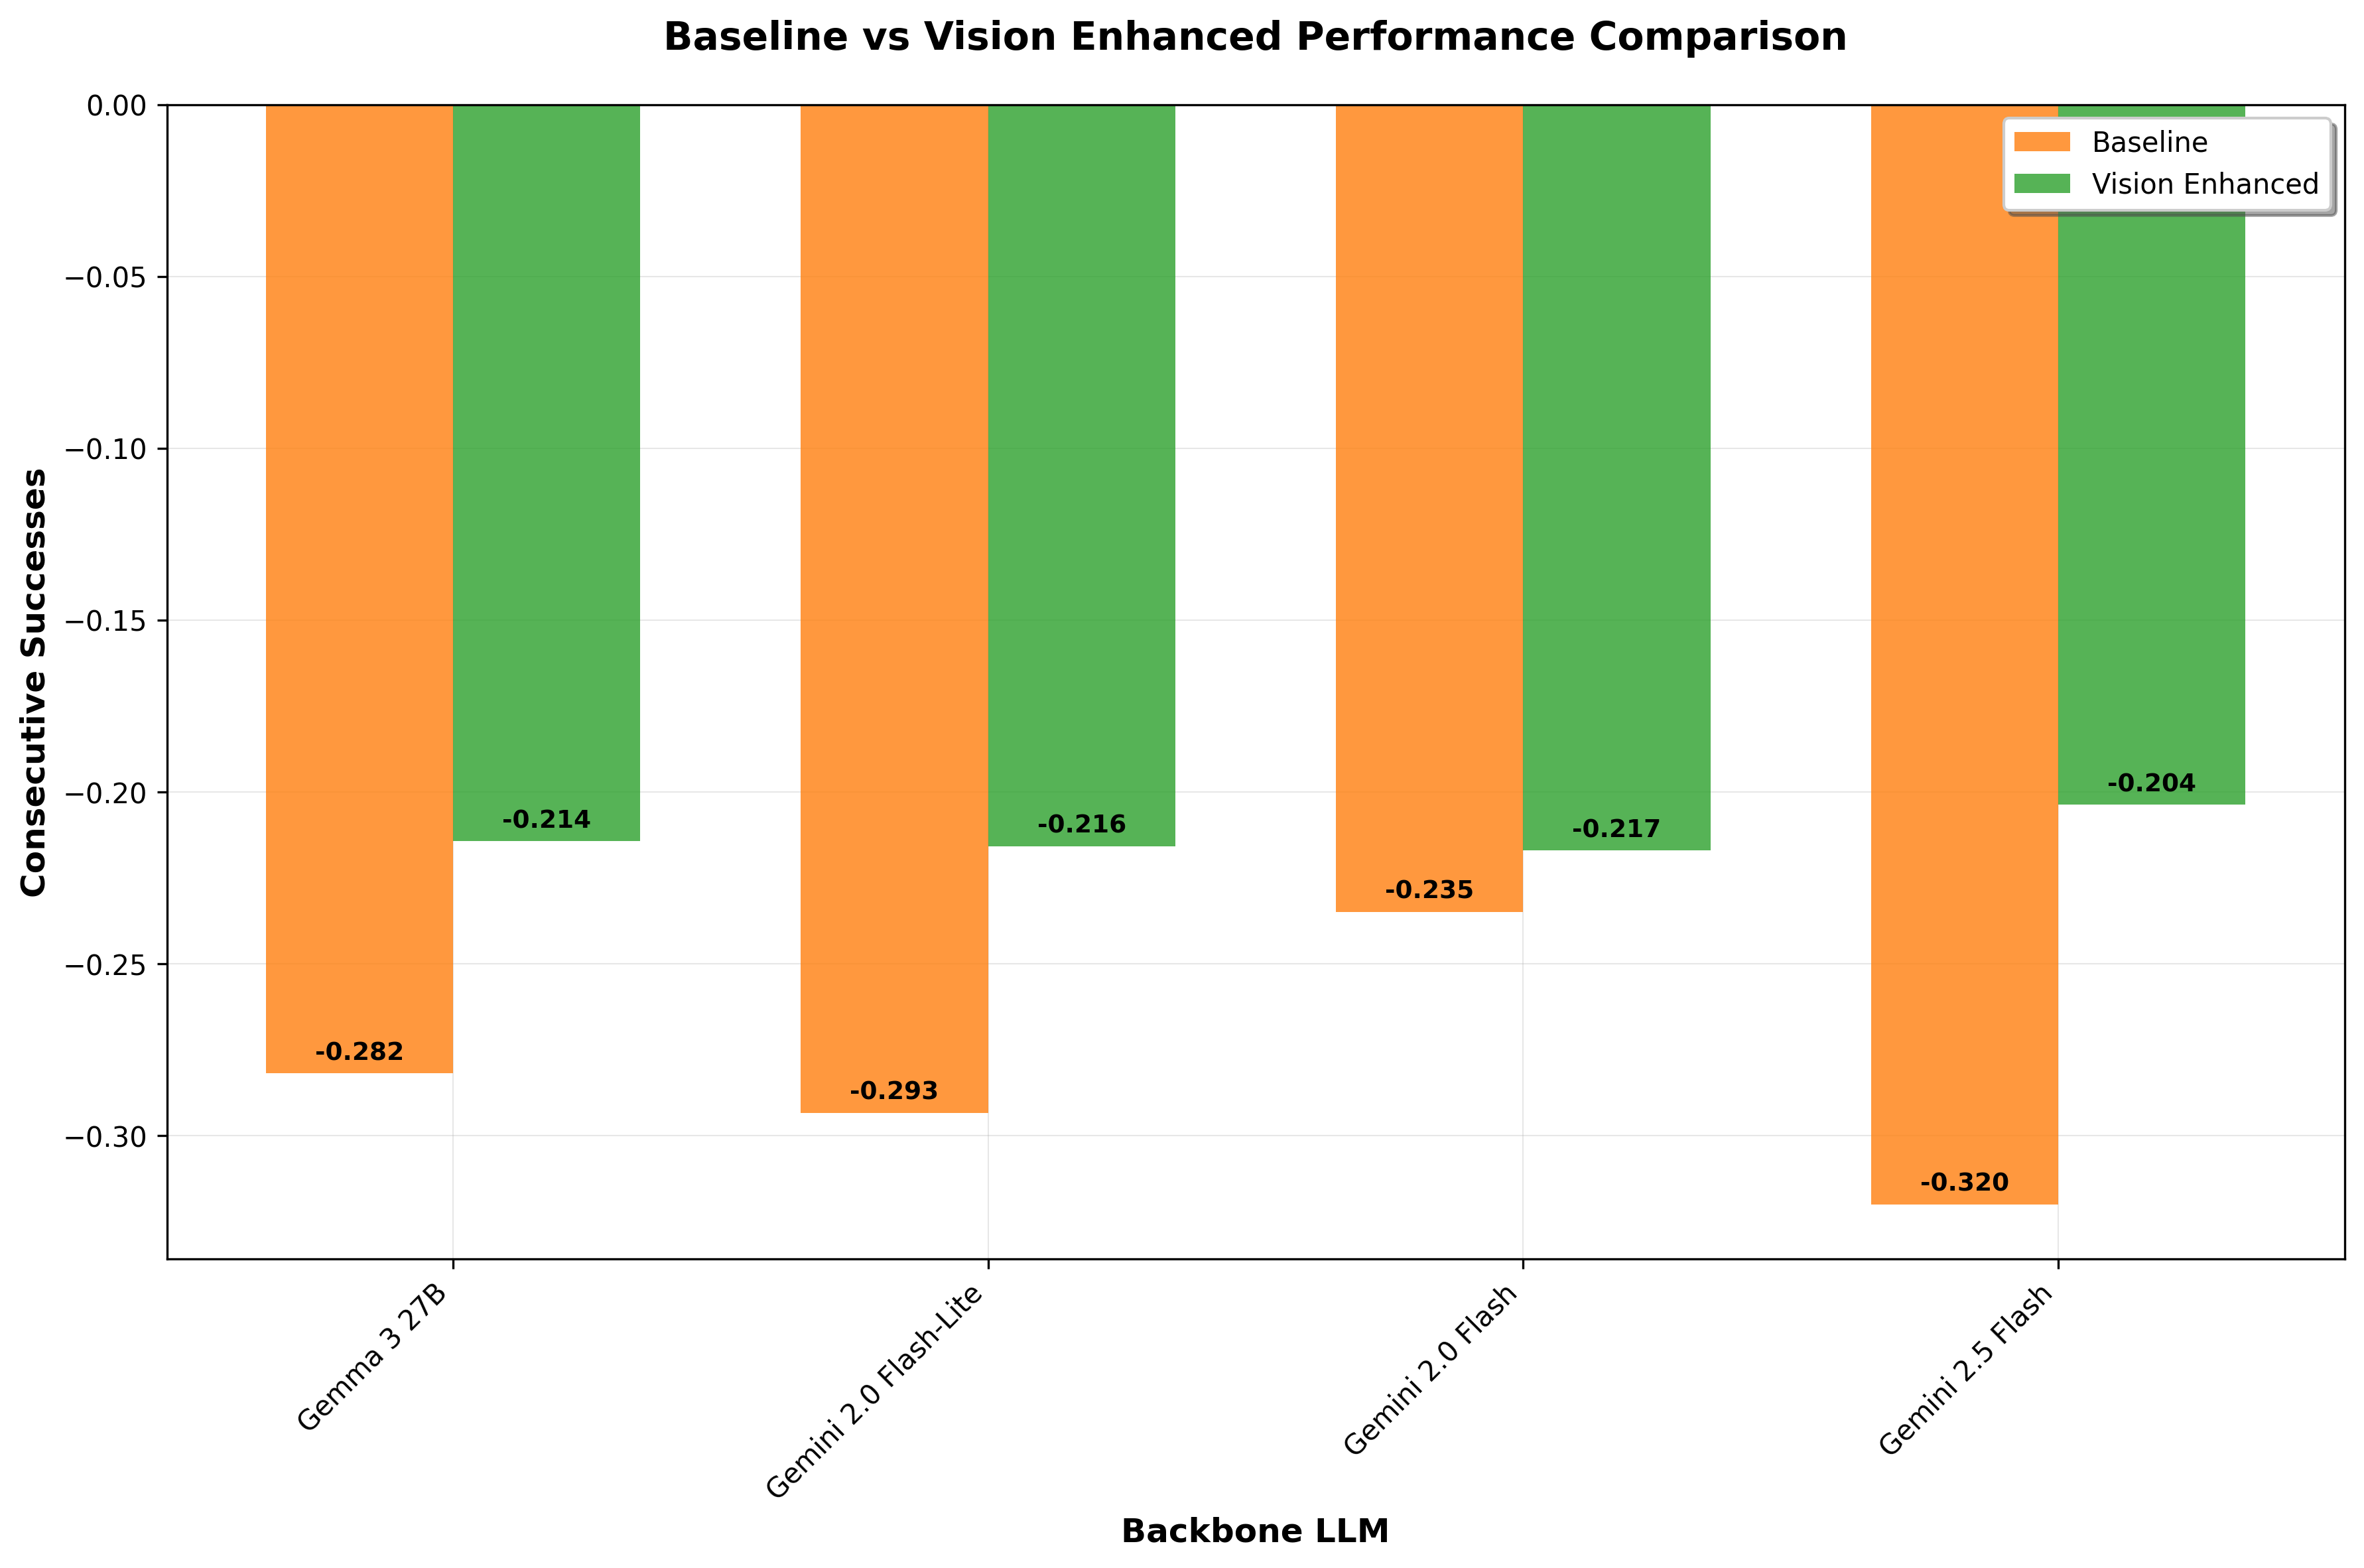
\includegraphics[width=1\linewidth]{baseline_vs_vision_model_comparison.png}
    \caption{Comparison of mean consecutive successes metric calculated from five runs of the final evaluation. Higher values are better. }
    \label{fig:baseline_vision_model_comparison}
\end{figure}

The results of experiments performed in such a setup and compared with analogous baseline runs are shown in Figure \ref{fig:baseline_vision_model_comparison}. The metric tested here is again defined as consecutive successes.

This chart mostly highlights two things:

\begin{enumerate}
    \item The results obtained using the vision-enhanced setup are significantly better for each of the tested LLM backbones.
    \item The results obtained using the vision-enhanced setup are less variant and better align with the idea of ``the bigger the model, the better the results''.
\end{enumerate}

The first observation supports our hypothesis that enhancing the feedback loop with visual context may lead to more efficient reward functions. On the other hand, the second observation suggests that the generation process is more robust and thus stable, giving more predictable results.

\begin{figure}
    \centering
    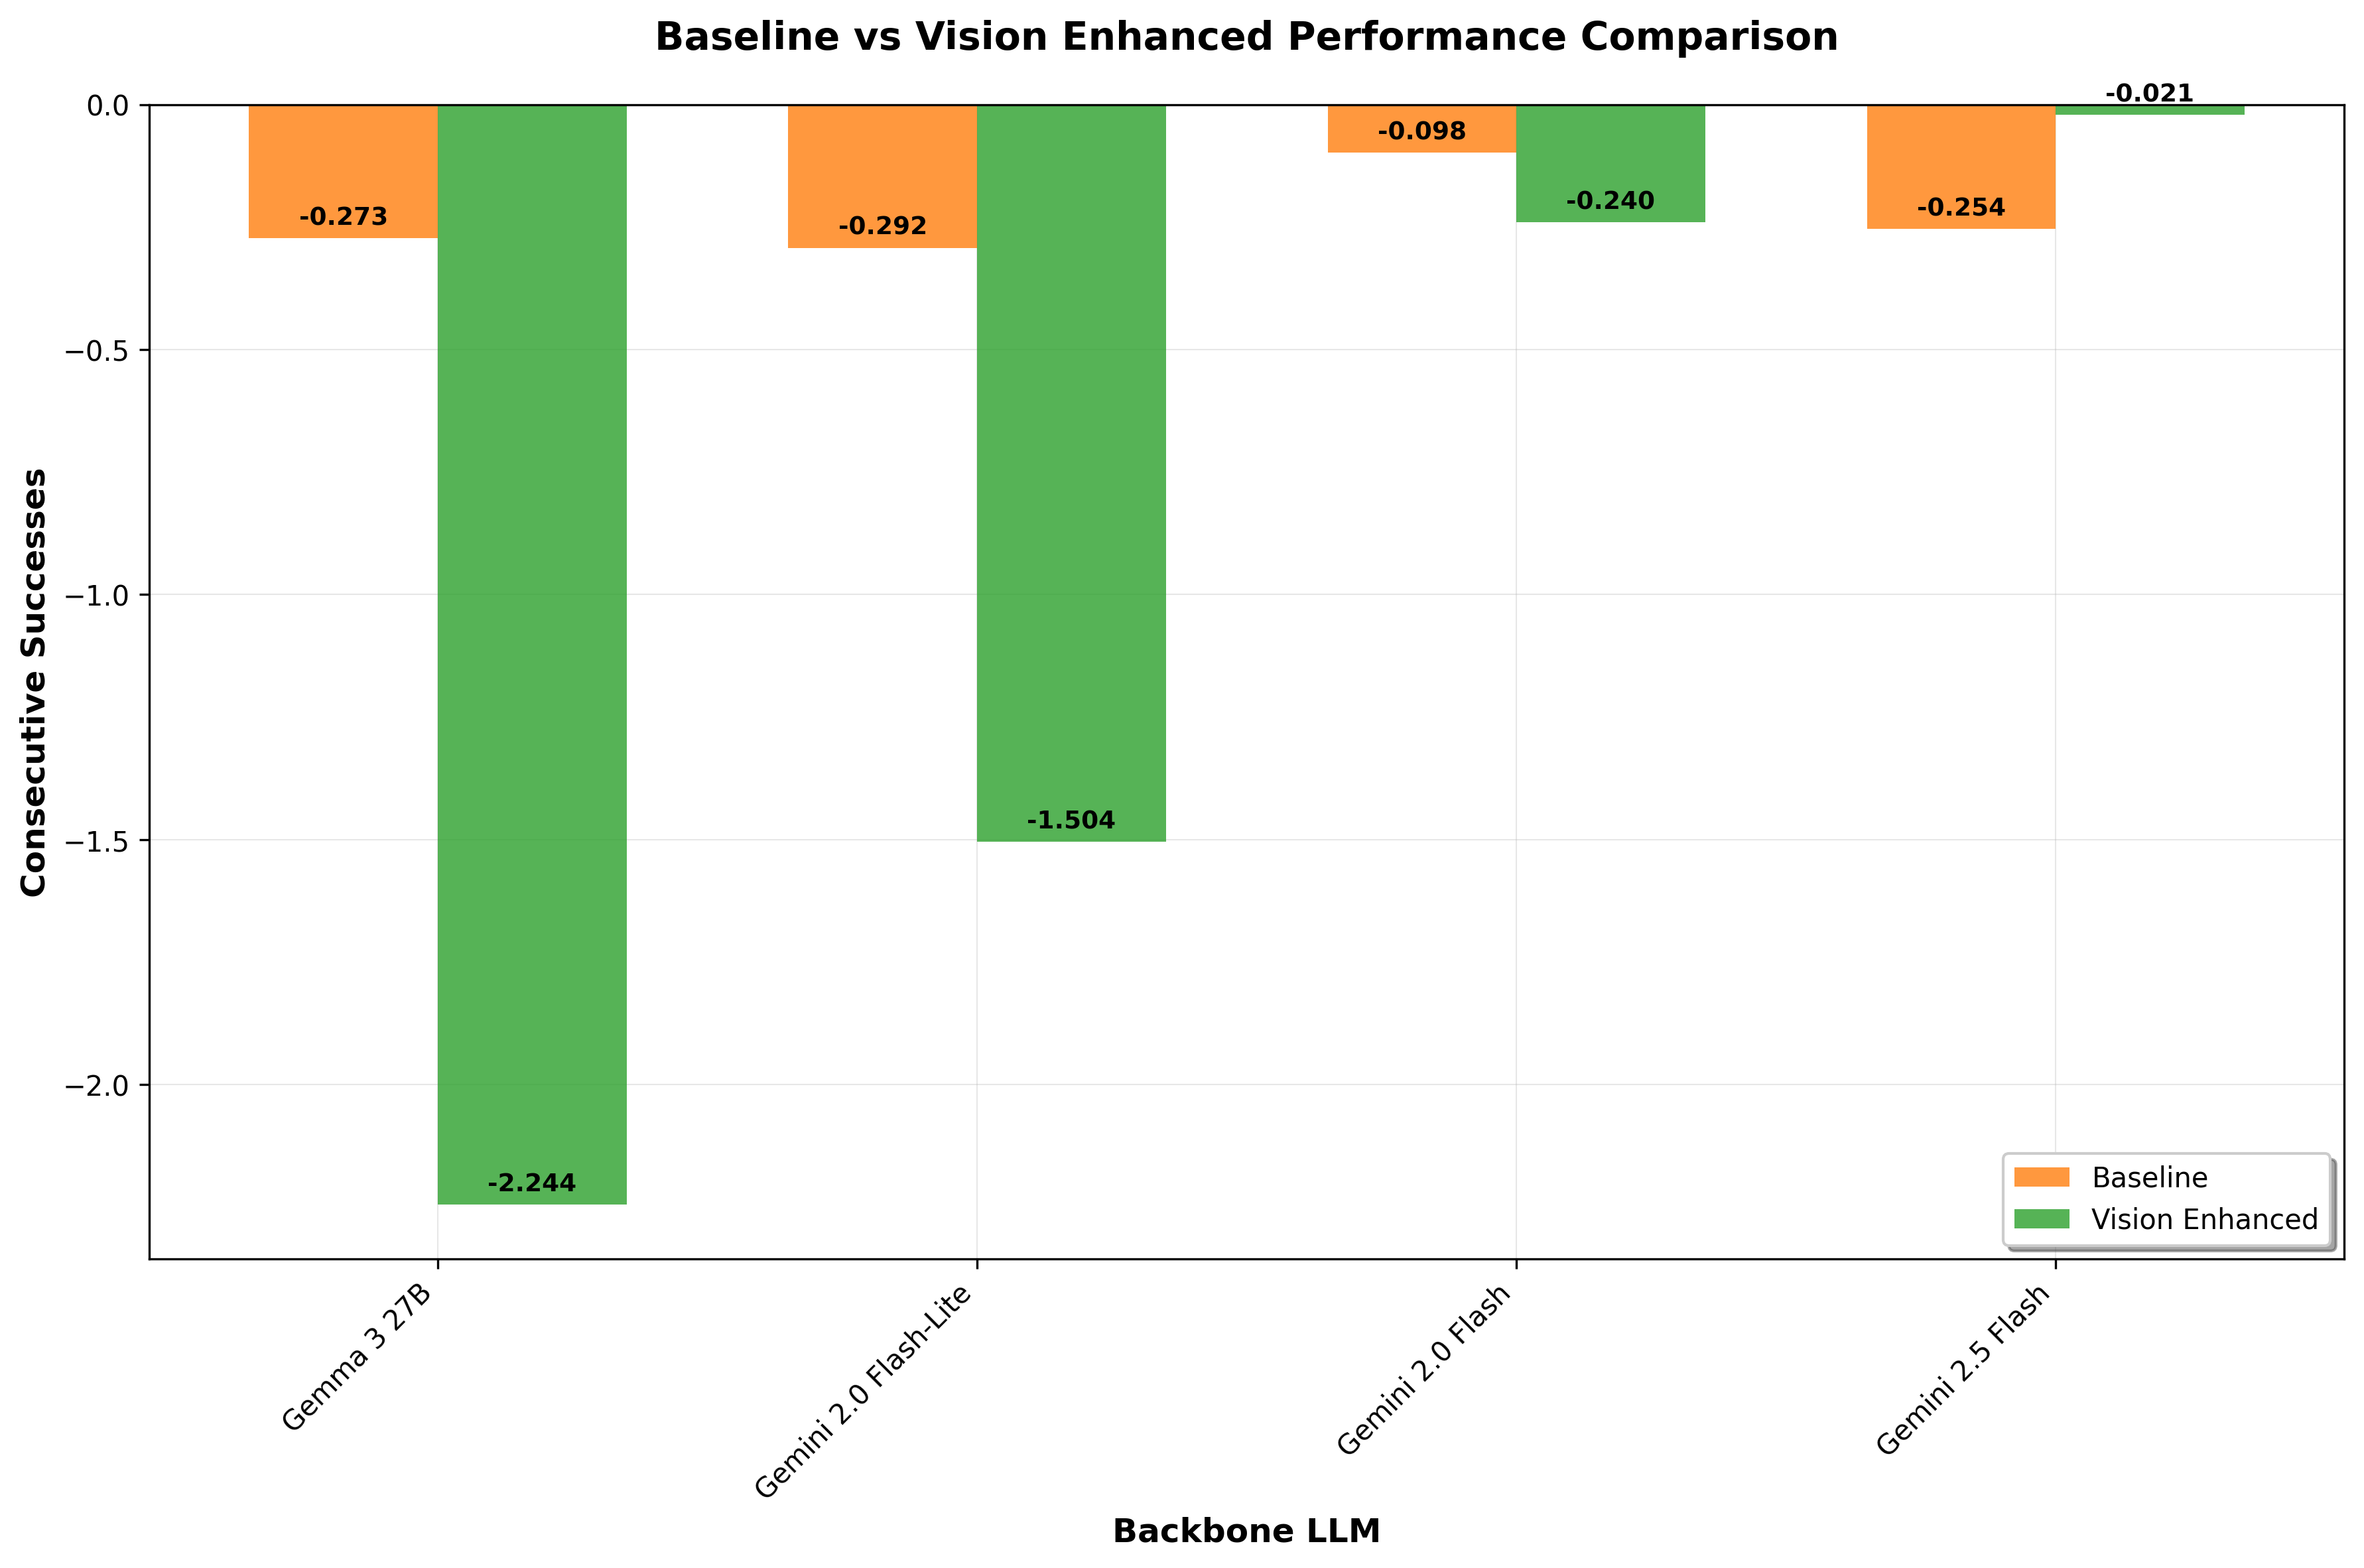
\includegraphics[width=1\linewidth]{baseline_vs_vision_extended_model_comparison.png}
    \caption{Comparison of final values of the extended setup of training for both baseline and vision-enhanced generations. Higher values are better.}
    \label{fig:baseline_vision_extended_model_comparison}
\end{figure}

To verify this further, we also compared both approaches in the extended variant of our training pipeline. Figure \ref{fig:baseline_vision_extended_model_comparison} shows the results of this comparison. Based on that, it's possible to draw some conclusions:

\begin{itemize}
    \item This setup further illustrates the positive correlation between model size and generated reward effectiveness. The difference is particularly striking between the smallest model (Gemma 3 27B) and the largest model (Gemini Flash 2.5).
    \item An interesting observation is that training powered by rewards generated by smaller models seems to diverge completely. This supports our hypothesis that these models are ineffective for such a challenging task.
    \item The benefits of using vision are not that obvious in this particular setup. For example, the results obtained for the Gemini 2.0 Flash were worse. However, we obtained an astonishingly near-perfect result using the Gemini 2.5 Flash model. The consecutive successes value of $-0.0208$ is better than any result obtained in previous experiments, and also better than the value resulting from the human-shaped reward.
    \item On the other hand, when we ran a simulation using the policy trained with the reward function generated by Gemini 2.5 Flash, we found that although the numerical value was almost perfect, the resulting movement pattern was very strange, causing the quadruped robot to ``slide'' forward instead of walking. It seemed as though the model had exploited the imperfect environment to achieve outstanding metric values by hacking the reward function. This also suggests that, although the consecutive successes metric is not flawed as we first suspected, it is also not perfect and favours setups that would definitely be deemed unsuccessful by a human evaluator vs the human-shaped, reward-powered policies that allow for far more natural movements.
\end{itemize}

\section{Conclusions}

\begin{thebibliography}{9}
\bibitem{eureka}
Yecheng Jason Ma and William Liang and Guanzhi Wang and De-An Huang and Osbert Bastani and Dinesh Jayaraman and Yuke Zhu and Linxi Fan and Anima Anandkumar, \emph{Eureka: Human-Level Reward Design via Coding Large Language Models}. arXiv preprint: Arxiv-2310.12931, 2023
\bibitem{l2r}
Wenhao Yu, Nimrod Gileadi, Chuyuan Fu, Sean Kirmani, Kuang-Huei Lee, Montse Gonzalez Arenas, Hao-Tien Lewis Chiang, Tom Erez, Leonard Hasenclever, Jan Humplik, et al. \emph{Language to rewards for robotic skill synthesis}. arXiv preprint arXiv:2306.08647, 2023.
\bibitem{isaac_gym}
Viktor Makoviychuk, Lukasz Wawrzyniak, Yunrong Guo, Michelle Lu, Kier Storey, Miles Macklin,
David Hoeller, Nikita Rudin, Arthur Allshire, Ankur Handa, et al. \emph{Isaac gym: High performance
gpu-based physics simulation for robot learning}. arXiv preprint arXiv:2108.10470, 2021.
\bibitem{eureka_repo}
Yecheng Jason Ma and William Liang, \emph{Eureka Repository on GitHub}, https://github.com/eureka-research/Eureka

\bibitem{ksim_repo}
K-Scale Labs, \emph{K-Sim Repository on GitHub}
https://github.com/kscalelabs/ksim

\bibitem{GPT-4}
OpenAI,
\href{https://arxiv.org/abs/2303.08774}{\emph{Gpt-4 technical report}},
Preprint,
arXiv:2303.08774.

\bibitem{Microsoft}
N. Wake, A. Kanehira, K. Sasabuchi, J. Takamatsu and K. Ikeuchi,
\href{https://ieeexplore.ieee.org/document/10235949}{\emph{ChatGPT Empowered Long-Step Robot Control in Various Environments: A Case Application}},
in IEEE Access, vol. 11, pp. 95060-95078, 2023,
doi: 10.1109/ACCESS.2023.3310935.

\bibitem{Nature}
Mon-Williams, R., Li, G., Long, R. et al.
\href{https://doi.org/10.1038/s42256-025-01005-x}{\emph{Embodied large language models enable robots to complete complex tasks in unpredictable environments.}}
Nat Mach Intell 7, 592–601 (2025).

\bibitem{TUDelft}
L.E. Verbaan et al.
\href{https://repository.tudelft.nl/record/uuid:2944a8e1-0a54-492b-af63-193a7ac11db8#title}{Perception and Control with Large Language Models in Robotic Manipulation}
Master Thesis at TUDelft, 2024

\bibitem{Gemini}
Gemini Team Google,
\href{https://arxiv.org/abs/2312.11805}{\emph{Gemini: A Family of Highly Capable Multimodal Models}},
arXiv:2312.11805

\bibitem{card}
Shengjie Sun, Runze Liu, Jiafei Lyu, Jing-Wen Yang, Liangpeng Zhang, Xiu Li,
\href{https://doi.org/10.48550/arXiv.2410.14660}{\emph{A Large Language Model-Driven Reward Design Framework via Dynamic Feedback for Reinforcement Learning}.}
arXiv:2410.14660, 2024

\bibitem{Text2Reward}
Tianbao Xie, Siheng Zhao, Chen Henry Wu, Yitao Liu, Qian Luo, Victor Zhong, Yanchao Yang, Tao Yu,
\href{https://doi.org/10.48550/arXiv.2309.11489}{\emph{Text2Reward: Reward Shaping with Language Models for Reinforcement Learning}},
arXiv:2309.11489 2023,

\bibitem{Gemma3-27B-IT}
Gemma Team,
\href{https://arxiv.org/abs/2503.19786}{\emph{Gemma 3 Technical Report}},
arXiv:2503.19786
Model Technical Report

\bibitem{Gemini_2.0_Flash}
Gemini Team,
\href{https://storage.googleapis.com/model-cards/documents/gemini-2-flash.pdf}{\emph{Gemini 2.0 Flash Model Card}},
Model Card

\bibitem{Gemini_2.0_Flash_Lite}
Gemini Team,
\href{https://storage.googleapis.com/model-cards/documents/gemini-2-flash-lite.pdf}{\emph{Gemini 2.0 Flash Model Card}},
Model Card

\bibitem{Gemini_2.5}
Gemini Team,
\href{https://storage.googleapis.com/deepmind-media/gemini/gemini_v2_5_report.pdf}{\emph{Gemini 2.5 Technical Report}},
Model Technical Report

\end{thebibliography}

\end{document}